
~\\~
\section{Examples} \label{sec:examples}
\enlargethispage{2\baselineskip} % Ensure no RIGHINO on newpage!
% [\TODO Here I could actually report, in a more detailed way, an example of how resource awareness was achieved on HPX: e.g. by reporting task grain size adaptivity by Grubel \cite{grubel2016dynamic}]

% [\TODO Here ideally report on how cfd-lab was ported to HPX]

% The code example reported here is based on assignments of the Parallel Programming course. I have implemented this solution with HPX as an alternative to the one based on PThreads required by that course.

\subsection{Mandelbrot set}
Drawing the Mandelbrot set is a classical example of an \emph{embarassingly parallel} problem, i.e. a problem which can be parallelized with little or no dependency between the parallel components. In this case there is no dependency at all, since each pixel can be computed independently from the others.

However, pixels belonging to the set and pixels at different distances from the boundary require different computational efforts to be drawn\footnote{Deciding whether a complex number belongs to the Mandelbrot set is done by checking if an associated sequence converges: where the sequence diverges faster, the point is quickly marked as external, while where the divergence is slower or where the sequence converges, it takes longer before a decision is reached.}, causing the parallel tasks to be potentially unbalanced.

\begin{figure}[h]
 	\begin{center}
 		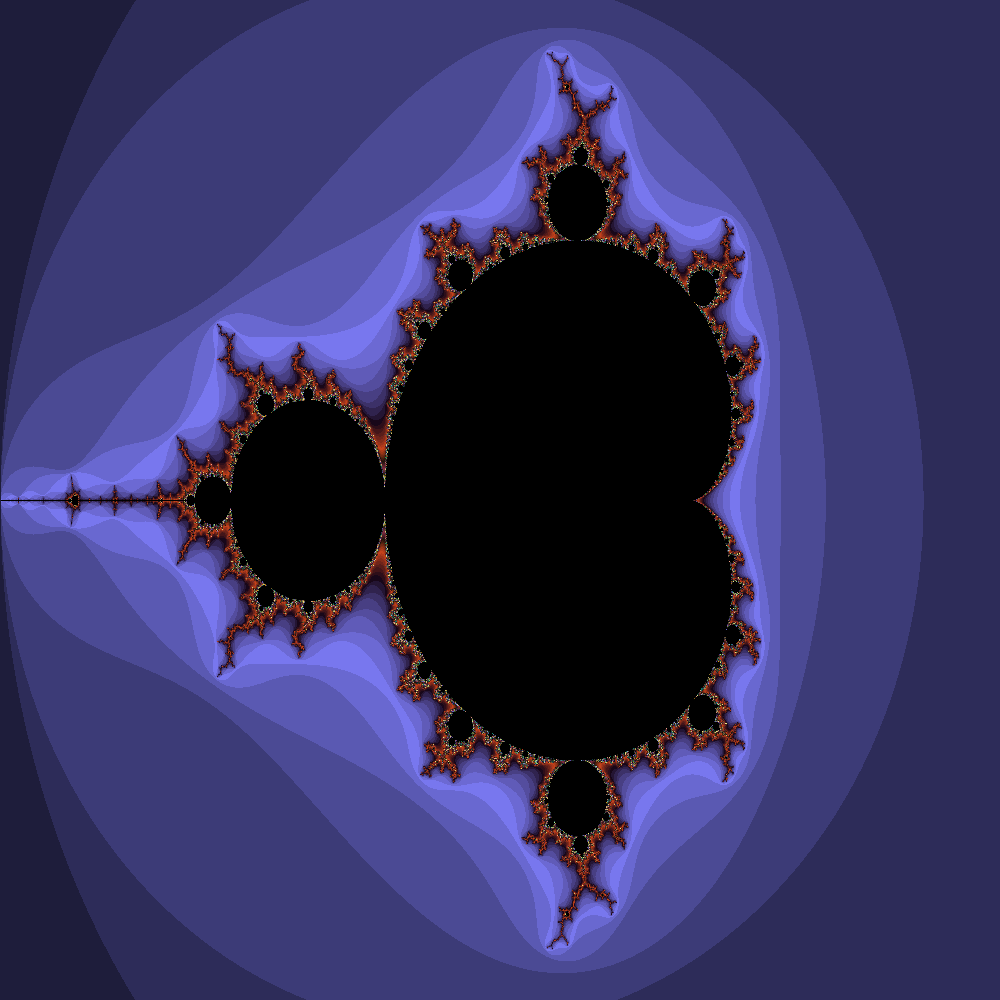
\includegraphics[scale=0.2]{Figures/mandelbrot.png}
 		\caption{An image of the Mandelbrot set generated by the code in this example.}
 		\label{fig:mandelbrotSet}
 	\end{center}
\end{figure}

Usually the image is split into ``slices'' containing a certain number of rows or columns of the image and each of these slices is assigned to a thread. Within a given slice the computation is performed pixel-by-pixel, sequentially.
The traditional way to ensure load balancing in a PThreads implementation is to split the image into small slices and to assign one of these to each thread; as soon as a thread finishes processing its slice, it gets a new one and proceeds further.
This requires additional code for managing how threads can get new work to do and it also requires synchronization, to ensure that no two threads get the same slice to process.

The implementation with HPX is much simpler: for each row of the image an \verb:async: call of the compute kernel is performed and the resulting future is stored into a vector. When all the asynchonous tasks have been created, \verb+hpx::wait_all+ is called on the vector of futures, making sure all tasks are completed before exiting.

I have tested strong scaling\footnote{How runtime improves by increasing the number of threads for a fixed problem size.} on the HPX- and PThread-based versions, with different problem sizes. I have also implemented and tested, for comparison purpose, a simple OpenMP-based version, which just parallelizes the outer loop (the row-loop). It uses dynamic scheduling for load balancing and a stride of 1 for consistency with the task grain size used with HPX.

The machine where I performed the tests has two sockets with 10 cores each, with each core exposing 2 hyperthreads. Unfortunately the machine was shared with other jobs, meaning that tests performed with a high number of threads have surely experienced preemption by the OS, artificially increasing their runtime.
However, this test is meant to roughly compare the three implementations and not to give an accurate measure on HPX's scaling capabilities. Keeping this and the aforementioned caveat in mind, we can see (Figure \ref{fig:speedupComparison}) how the performance of the HPX-based implementation is on par with the optimized PThreads-based one. On the other end we can also see how following the same approach with OpenMP does not yield the same performance: one possible explanation is that the relatively small task grain size chosen causes a relevant overhead in OpenMP.

This is clearly a toy example but it shows how HPX allows achieving good performance with simple and clean code and without any explicit optimization effort. Programmability is an important factor for making parallelism more accessible and this is surely one of the strengths of HPX.
% and neither the HPX nor the PThreads implementations have been optimized and tuned for achieving the maximum possible performance. However a certain effort was required in order to get the PThreads version right
~\\~

\subsection{Reading performance counters from the command line}
Although it is possible to access performance counter data from within the application, using the HPX API, it is also possible to make the HPX runtime print data from any performance counter to the commandline. This can be useful for debugging or for manual tuning of an HPX application.

This is achieved by passing extra flags to an HPX application and is completely handled by the runtime system, thus not requiring any change in the application code.

Available counters can be listed using the \verb/--hpx:list-counters/ flag and, if HPX was built with PAPI\footnote{Performance Application Programming Interface, which allows accessing hardware counters.} support, available PAPI events can be listed with \verb/--hpx:papi-event-info=all/.

A counter can be printed by passing the \verb/--hpx:print-counter='<counter_name>'/ argument and several counters may be specified at the same time by passing this argument multiple times.
This makes the HPX runtime system print the specified counters at the end of the execution. It is also possible to have the counters printed at regular time intervals during execution by adding the \verb/--hpx:print-counter-interval=<interval_ms>/ argument, where the interval is expressed in milliseconds.
% [\TODO Here add a couple of easy examples on how to parallelize using HPX tasks and an example on how to read a performance counter].
\begin{figure}[t]
 	\begin{center}
 		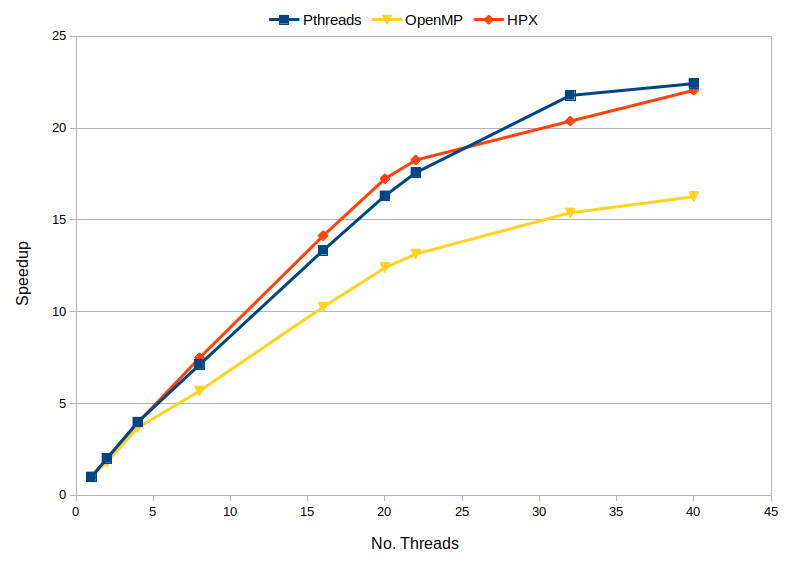
\includegraphics[scale=0.40]{Figures/mandelbrot_speedup_comparison.png}
 		\caption{Speedup comparison for PThreads, OpenMP and HPX implementations
 		% with respect to the sequential version 
 		on a $10^4$x$10^4$ image. Both the OpenMP and HPX versions use the basic features of the respective runtime system, meaning a parallelization on the row-loop (with dynamic scheduling) and an asynchronous execution for each row of the image respectively. The PThreads version instead includes a more complex logic to ensure load balancing between the threads. The results show how the HPX implementation, using basic syntax and without any specific tuning, is able to perform on par with a specifically optimized PThreads implementation. All three implementations use the same task grain size consisting of one image row.}
 		\label{fig:speedupComparison}
 	\end{center}
\end{figure}

%eof
